\documentclass[11pt]{article}

% ============================================================================
% TITLE (working):
%   "One Attention Layer Is Enough: Diagnosing and Repairing State-Space
%    Encoders for Routing under Reinforcement Learning"
% Alternatives (comments only):
%   (A) "Serpentine Routing: When a Linear-Scan Encoder Needs One Attention
%        Layer to Match Transformers on TSP under RL"
%   (B) "Diagnosing the State-Space Encoder Gap in Neural Combinatorial
%        Optimization: Direction, Order, and a Single Attention Layer"
% ============================================================================

\usepackage[utf8]{inputenc}
\usepackage[T1]{fontenc}

% --- Page geometry: arXiv/NeurIPS-preprint margins ---
\usepackage[letterpaper,margin=1in]{geometry}

% --- Math and symbols ---
\usepackage{amsmath,amssymb}

% --- Typography: Times-like text + matching math, with microtype refinements ---
\usepackage{newtxtext}
\usepackage{newtxmath}
\usepackage[protrusion=true,expansion=false,final]{microtype}
\linespread{1.04}

% --- Graphics, tables, floats ---
\usepackage{graphicx}
\usepackage{booktabs}
\renewcommand{\arraystretch}{1.18}
\usepackage[font=small,labelfont=bf,labelsep=period,skip=6pt]{caption}

% --- Section heading styling (modest, no color) ---
\usepackage{titlesec}
\titleformat{\section}{\normalfont\large\bfseries}{\thesection}{0.75em}{}
\titleformat{\subsection}{\normalfont\normalsize\bfseries}{\thesubsection}{0.6em}{}
\titlespacing*{\section}{0pt}{2.4ex plus 1ex minus .2ex}{1.2ex plus .2ex}
\titlespacing*{\subsection}{0pt}{2.0ex plus .8ex minus .2ex}{0.9ex plus .2ex}

% --- References and links ---
\usepackage{natbib}
\usepackage{url}
\usepackage{hyperref}
\usepackage{xcolor}
\usepackage{authblk}

\hypersetup{colorlinks=true, linkcolor=blue!50!black, citecolor=blue!50!black, urlcolor=blue!50!black}

% --- Title-block spacing ---
\renewcommand\Authfont{\normalsize\scshape}
\renewcommand\Affilfont{\normalsize\itshape}
\setlength{\affilsep}{0.6em}

\newcommand{\pct}{\%}

\title{When Mamba Needs Attention}

\author{Umar Aslam\thanks{Independent Researcher. Correspondence: \texttt{umaraslam66@hotmail.com}.}}
\affil{Independent Researcher}
\date{}

\begin{document}
\maketitle

\begin{abstract}
We ask whether a linear-time state-space (Mamba) encoder can drive routing
decisions as well as a quadratic-time attention encoder on Euclidean TSP-100,
under identical POMO reinforcement learning and a byte-identical decoder, with
only the encoder swapped and parameter counts matched.\footnote{Code and
pre-registered decision rules: \url{https://github.com/Umaraslam66/serpentine}.}
The obvious recipe---a Hilbert-curve serialization scanned by a unidirectional
Mamba---is killed: at a matched 250k-step budget it reaches a 7.50\,$\pm$\,1.03
single-trajectory optimality gap over three seeds (8.34\pct{} on the
pre-registered seed) versus attention's 2.95\pct. Diagnostics
localize the failure to a short, one-directional receptive field rather than a
wiring bug or representation collapse, and a geometry study shows the Hilbert
prior scatters $\sim$14\pct{} of spatial neighbors far apart on the scan line.
An ordering ablation initially suggested a strict random $<$ sort $<$ Hilbert
inversion, but two further seeds refuted the strict claim; the surviving,
scoped statement is that a locality prior confers no benefit for \emph{causal}
scans and roughly doubles seed variance ($\sigma$ 1.03 vs 0.53). Repair follows
the diagnosis: pooled global channels fail, but a param-matched bidirectional
scan reaches multistart parity with attention (1.94\,$\pm$\,0.09 vs 1.91) and
cuts seed variance tenfold, and a hybrid inserting \emph{one} attention layer
into a bidirectional-Mamba stack (4.5\pct{} fewer parameters) beats attention on
multistart tour quality at a converged 500k budget (worst hybrid seed 1.365 $<$
best attention 1.589). All claims are scoped to N$=$100; the O(N) payoff remains
untested.
\end{abstract}

% ============================================================================
\section{Introduction}
% ============================================================================

Neural constructive solvers for routing problems build a tour one node at a
time, and the dominant architecture is an attention encoder followed by an
attention-based autoregressive decoder \citep{kool2019,pomo2020}. The encoder's
job is to embed each city so that the decoder can compare candidates; attention
gives every node an all-pairs view of the instance at $O(N^2)$ cost per layer.
State-space models such as Mamba \citep{mamba2023,s4-2022} process a sequence in
$O(N)$ time with a selective linear recurrence, and have become a competitive
backbone for point clouds \citep{pointmamba2024,ptv3-2024,pcm2025}. This raises
a concrete question for neural combinatorial optimization (NCO): \emph{can an
$O(N)$ state-space encoder route as well as an $O(N^2)$ attention encoder, under
the reinforcement-learning training that NCO actually uses?}

We treat this as a fail-fast experiment. We fix the decoder, the training
algorithm (POMO REINFORCE \citep{pomo2020,williams1992}), the optimizer, the
budget, the evaluation set, and the parameter count, and swap only the encoder.
A state-space encoder needs a serialization---an order in which to scan the
unordered node set---and the natural choice for 2D points is a space-filling
Hilbert curve \citep{hilbert1891,ptv3-2024}. The candidate is therefore a
Hilbert-ordered unidirectional Mamba encoder; we ask whether it clears the
attention baseline.

It does not. We then use the failure as a diagnostic object rather than a dead
end, and follow the mechanism to a repair. Our contributions, scoped honestly:

\begin{itemize}
  \item \textbf{A clean kill of the vanilla recipe under RL.} At matched
  parameters and budget on TSP-100, a Hilbert-ordered unidirectional Mamba
  encoder reaches a 7.50\,$\pm$\,1.03 single-trajectory gap across three seeds
  (its \emph{best} seed, 6.36\pct, is still more than 3 points behind
  attention's 2.95\pct; \S\ref{sec:kill}). The kill was pre-registered.
  \item \textbf{A localized diagnosis.} The failure is not a wiring bug (order
  demonstrably reaches the decoder) and not representation collapse (the Mamba
  embeddings are higher-rank than attention's); finite-difference probes show a
  short, strictly causal receptive field, and a model-free geometry study shows
  the Hilbert prior scatters $\sim$14\pct{} of spatial neighbors (\S\ref{sec:kill}).
  \item \textbf{A methodological finding about ordering priors and seeds.} A
  single-seed ablation suggested a strict random $<$ sort $<$ Hilbert inversion;
  two further seeds refuted the strict claim. The surviving statement is that a
  locality prior buys nothing for \emph{causal} scans and doubles seed variance,
  and---crucially---that its value depends on scan causality: with a bidirectional
  scan, random ordering \emph{hurts} (\S\ref{sec:order}).
  \item \textbf{A diagnosis-guided repair.} Pooled global channels do not help
  under RL; a param-matched bidirectional scan reaches multistart parity with
  attention and stabilizes training tenfold; and a hybrid with a single attention
  layer beats attention on converged multistart tour quality with fewer
  parameters (\S\ref{sec:repair}).
  \item \textbf{A decode-diversity observation attention lacks.} Because a scan
  encoder has an ordering degree of freedom, best-of-$k$ serialization ensembling
  at inference improves tour quality for free; attention has no such knob
  (\S\ref{sec:repair}).
\end{itemize}

We are careful about novelty. Bidirectional scans, space-filling serializations,
and SSM--attention hybrids are all prior art in the point-cloud and language-model
literatures (\S\ref{sec:related}); what is new here is the controlled,
matched-budget evidence for \emph{routing decisions under policy-gradient RL at
N$=$100}, and the contrast between exact sparse attention and pooled global
channels as repairs.

% ============================================================================
\section{Related work}
\label{sec:related}
% ============================================================================

\paragraph{Neural combinatorial optimization.}
Pointer networks introduced sequence-to-sequence attention for combinatorial
outputs \citep{pointernet2015}; \citet{bello2016} trained such models with
reinforcement learning; \citet{kool2019} established the attention-encoder /
attention-decoder template for routing, and POMO \citep{pomo2020} added
multiple-optima rollouts with a shared baseline and instance augmentation. Our
training and evaluation follow POMO; classical LKH-3 \citep{lkh3} provides the
optimality oracle.

\paragraph{State-space models.}
Structured state-space models \citep{s4-2022} and the selective Mamba
variant \citep{mamba2023} give $O(N)$ sequence modeling with a linear recurrence,
and are the backbone we test as an encoder. Mamba has also been applied to RL as
offline trajectory modeling \citep{decisionmamba2024}, a different problem from
the constructive routing we study.

\paragraph{Mamba for point clouds.}
Mamba has been adapted extensively to unordered 3D points, which, like routing,
require serializing a set. The canonical observation that a unidirectional scan
has a causal, all-pairs-free receptive field relative to attention is from
PointMamba \citep{pointmamba2024}. Known mitigations---all prior art---include
bidirectional scanning \citep{vim2024,hydramamba2025,pamba2025}, multi-curve or
shuffled serialization \citep{ptv3-2024}, and hybrid local/global aggregation
\citep{pillarmamba2025}. HydraMamba \citep{hydramamba2025} further notes that a
bidirectional scan still compresses history into a finite hidden state, which is
why we expect bidirectionality to close the gap only partially. Point Cloud
Mamba \citep{pcm2025} reports that simple orders are roughly on par with
space-filling curves. We reuse this diagnostic vocabulary; we do not claim it.

\paragraph{Mamba for combinatorial optimization.}
ECO \citep{eco2026} applies a Mamba encoder--decoder to TSP/CVRP, but trains via
supervised fine-tuning plus iterative preference optimization (not
policy-gradient RL), targets large instances (its smallest reported TSP is
N$=$200), and never tests N$=$100. The cell we occupy---matched-budget POMO
REINFORCE at N$=$100, decoder held fixed---is not covered by ECO, and our kill of
vanilla Mamba+Hilbert at N$=$100 is consistent with ECO's large-N focus and its
reliance on supervised bootstrapping.

\paragraph{Hybrid SSM--attention models.}
Interleaving attention layers into an SSM backbone is established in language
models: Jamba \citep{jamba2024} and Zamba \citep{zamba2024} both mix Mamba and
attention blocks for efficiency. Our hybrid uses the same idea; the contribution
is not the interleaving pattern but the RL-routing evidence that \emph{one} exact
attention layer succeeds where pooled global channels fail.

% ============================================================================
\section{Setting}
\label{sec:setting}
% ============================================================================

\paragraph{Problem and data.}
We study the Euclidean Traveling Salesman Problem with $N=100$ nodes drawn
i.i.d.\ uniformly from $[0,1]^2$. Evaluation uses a fixed held-out set of 1000
instances; the oracle is LKH-3 \citep{lkh3} with mean optimal tour length
$7.749371521$. All gaps are reported as percent excess over this oracle mean.

\paragraph{Training.}
Every encoder is trained with POMO policy-gradient RL \citep{pomo2020}: REINFORCE
with a shared-baseline advantage equal to the reward minus the per-instance mean
over 100 POMO rollouts. The decoder (the POMO TSP decoder) is byte-identical
across all encoders; only the encoder is swapped. We use Adam with learning rate
$1\times10^{-4}$, weight decay $1\times10^{-6}$, batch size 64, and 250k gradient
steps (500k for the converged extensions). Each run uses a single
NVIDIA~A100-SXM-64GB on the CINECA Leonardo Booster.

\paragraph{Evaluation protocol.}
We report two metrics. \emph{Single-trajectory} gap is greedy argmax decoding
averaged over the 100 POMO start nodes. \emph{Multistart} gap is the best of the
100 start-node rollouts, with \emph{no} instance augmentation. We deliberately
omit the $\times$8 augmentation used in headline POMO numbers so that the
encoder, not the augmentation, is what the comparison measures.

\paragraph{Relation to published POMO numbers.}
Published POMO reaches $\sim$1\pct{} greedy on TSP-100 at a much larger training
budget; we reproduced the official released checkpoint at 0.97\pct{} greedy
(0.149\pct{} with $\times$8 augmentation) under our exact oracle and evaluation
set as a seatbelt before any experiment (artifact in the repository). Our
attention baseline is therefore not undertrained relative to its budget---it is
the same architecture trained at a deliberately smaller, \emph{matched} budget
(250k steps of batch 64, $\approx$16M instances), because every claim in this
paper is a matched-budget comparison between encoders, not a state-of-the-art
claim. Absolute gaps here should not be compared against headline POMO numbers.

\paragraph{Parameter matching.}
The encoders are matched in total model size to within 4.5\pct{}
(Table~\ref{tab:params}): attention
(6 layers, $d=128$, 8 heads) totals 1{,}269{,}760 parameters; the unidirectional
Mamba encoder (10 Mamba-1 blocks, $d=128$) totals 1{,}249{,}792; the
bidirectional Mamba (5 layers, each summing a forward and backward scan) totals
1{,}248{,}512; and the hybrid (4 bidirectional-Mamba layers with one POMO-native
attention layer inserted after layer 2) totals 1{,}213{,}184---4.5\pct{}
\emph{fewer} parameters than attention. The Mamba runs use the mamba-ssm CUDA
kernel, gated against a pure-PyTorch reference at $<10^{-3}$ agreement.
Throughput on the A100 is comparable across encoders (attention $\sim$5.1,
unidirectional Mamba 5.03--5.04, bidirectional 4.78, hybrid $\sim$4.8 it/s).

\paragraph{Serialization.}
A scan encoder needs a node order. We serialize the nodes, scan, and
un-serialize back to the original node order before decoding. The default order
is the Hilbert curve; we also study a fresh random permutation per instance and a
coordinate (lexicographic) sort as ablation arms.

\begin{table}[t]
\centering
\caption{Encoder configurations, matched in total parameters. The hybrid has the
fewest parameters (4.5\pct{} below attention).}
\label{tab:params}
\small
\setlength{\tabcolsep}{5pt}
\begin{tabular}{lll r}
\toprule
Encoder & Layers & Serialization & Parameters \\
\midrule
Attention        & 6 (d=128, 8 heads)                       & --- (permutation-invariant) & 1{,}269{,}760 \\
Uni-Mamba        & 10 Mamba-1 blocks                        & Hilbert / random / sort & 1{,}249{,}792 \\
BiMamba          & 5 (fwd+bwd scan, summed)                 & Hilbert / random & 1{,}248{,}512 \\
Hybrid           & 4 BiMamba + 1 attention (after layer 2)  & Hilbert & 1{,}213{,}184 \\
\bottomrule
\end{tabular}
\end{table}

% ============================================================================
\section{The kill and the diagnosis}
\label{sec:kill}
% ============================================================================

\paragraph{The vanilla recipe is killed.}
Before running, we fixed a kill rule: kill the candidate if it is worse than
attention by more than 1 percentage point \emph{and} Hilbert clearly beats
random ordering. At the matched 250k-step budget the Hilbert-ordered
unidirectional Mamba reaches an 8.34\pct{} single-trajectory gap and 4.46\pct{}
multistart on the pre-registered seed (three-seed mean 7.50\,$\pm$\,1.03 /
3.64\,$\pm$\,1.09; even its best seed trails attention by more than 3 points),
versus attention's 2.95\pct{} / 1.91\pct{} (Table~\ref{tab:main}). The first
clause of the kill rule is satisfied by a wide margin under every seed; as
\S\ref{sec:order} shows, the second clause resolves in an unanticipated
direction. The encoder-swap-as-specified is dead. We now ask
\emph{why}, using four diagnostics on the trained Hilbert/uni-Mamba seed-1
checkpoint.

\paragraph{(1) It is not a wiring bug---order reaches the decoder.}
We swap the inference-time scan order on the trained checkpoint without
retraining, on an $n=200$ subset (hence the small offset from the $n=1000$
figures elsewhere). The gap moves from 8.38\pct{} (Hilbert, the training order)
to 33.49\pct{} (sort) to 56.38\pct{} (random). Feeding the wrong order collapses
the model, so the serialize$\rightarrow$scan$\rightarrow$un-serialize$\rightarrow$decode
path is intact and strongly order-dependent; the failure is not a plumbing bug.

\paragraph{(2) It is not representation collapse.}
On 10k node embeddings, the Mamba encoder has effective rank 31.7 (attention:
26.0), mean pairwise cosine similarity 0.116 (0.102), and zero dead dimensions
(as does attention). The embeddings are at least as healthy and high-rank as
attention's; the deficit is in \emph{what} they encode, not encoder health.

\paragraph{(3) The receptive field is short and one-directional.}
Finite-difference sensitivity shows that upstream sensitivity is exactly zero (a
node never sees its sequence-successors), and downstream influence decays
$\sim$99\pct{} within $\sim$20 sequence positions. Each node integrates only a
short, one-directional window---consistent with the causal-scan limitation of
PointMamba \citep{pointmamba2024}.

\paragraph{(4) The Hilbert prior scatters spatial neighbors.}
A model-free geometry study shows that at N$=$100 the Hilbert curve places
14.4\pct{} of each node's $k=5$ nearest 2D neighbors more than 10 sequence
positions apart on the scan line (curve-boundary discontinuities). A short causal
window cannot reconnect them, whereas all-pairs attention sees them for free. The
scatter worsens with scale: the mean line-separation of spatial neighbors grows
from 7 to 48 as $N$ grows from 100 to 5000 (fraction $>$10 apart:
14.6\pct{}$\rightarrow$22.2\pct{} under the scaling study's estimator, which
differs slightly from the 14.4\pct{} $k{=}5$ figure above), while the encoder's
receptive field is fixed ($\sim$20). This is a geometry of the serialization, not a contribution of ours;
it predicts the limitation \emph{worsens} at the larger $N$ where $O(N)$ would
otherwise pay off.

% ============================================================================
\section{Ordering ablation and the seed lesson}
\label{sec:order}
% ============================================================================

The second clause of the kill rule---"Hilbert clearly beats random"---turns out
to be false, and the way it turned out is itself a methodological lesson. We
trained unidirectional Mamba from scratch under three serializations, identical
in every other respect (Figure~\ref{fig:order}).

\paragraph{The seed-1 inversion.}
On seed 1, the ordering hierarchy inverted relative to the locality prior:
random 6.40\pct{} $<$ sort 7.12\pct{} $<$ Hilbert 8.34\pct{} single-trajectory,
with random ahead of Hilbert at every 20k-step checkpoint. Read literally, this
refutes the Hilbert-locality premise: spatial-locality serialization does not
help this encoder---it hurts.

\paragraph{Refutation by further seeds.}
Seeds 2--3 do not sustain the strict inversion. Across three seeds, Hilbert spans
6.36--8.34 (mean 7.50\,$\pm$\,1.03) and random spans 6.40--7.45
(mean 6.90\,$\pm$\,0.53); the ranges overlap, and Hilbert seed~2 in fact beats
every random seed. The strict "random $<$ sort $<$ Hilbert whole-curve" claim was
a seed-1 artifact and must not be stated unqualified.

\paragraph{The surviving claim.}
What survives is weaker and, we think, more useful: \emph{a locality prior
confers no measurable benefit over random ordering for a causal scan, and roughly
doubles run-to-run variance} ($\sigma$ 1.03 for Hilbert vs 0.53 for random). This
is closer to Point Cloud Mamba's "simple $\approx$ curve orders"
\citep{pcm2025} than to a strict inversion. The pre-registered expectation that
Hilbert would clearly beat random finds no support.

\paragraph{Causality-dependence.}
The value of a locality prior depends on scan causality. With the bidirectional
scan of \S\ref{sec:repair}, random ordering instead \emph{hurts}: BiMamba/random
reaches 7.61\pct{} versus BiMamba/Hilbert 5.57\pct{}. Mechanistically, once both
scan directions are available, Hilbert locality becomes exploitable structure and
random ordering destroys it; for a causal scan it is a crutch the short window
overfits. The one-line takeaway is that the "best" serialization is not a property
of the geometry alone but of the geometry \emph{and} the scan's directionality.

We frame this as a methodological finding as much as an empirical one: a
single-seed ordering curve, however cleanly separated, was enough to state an
inverted hierarchy that two further seeds dissolved. The pre-registered
decision rule survived the surprise only because the seed budget was part of the
plan.

\begin{figure}[t]
\centering
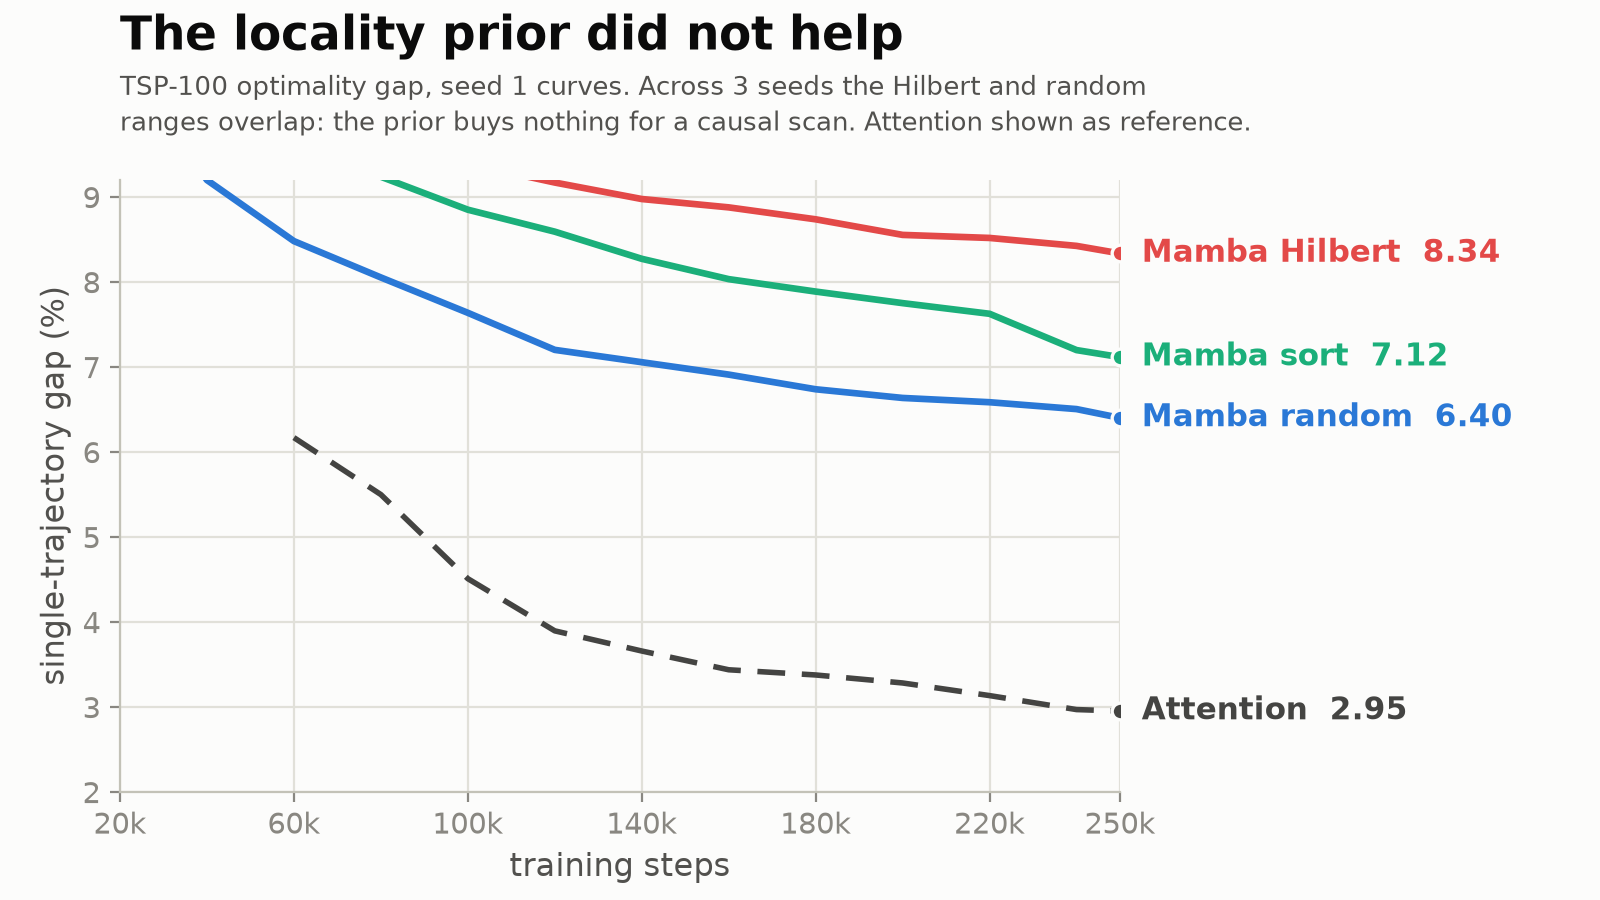
\includegraphics[width=0.85\linewidth]{figs/fig_ordering_curves.png}
\caption{Ordering ablation for the unidirectional Mamba encoder (single-trajectory
gap vs training step). On seed 1 the hierarchy separates as
random $<$ sort $<$ Hilbert at every checkpoint; seeds 2--3 (\S\ref{sec:order})
show the Hilbert and random distributions overlap. The surviving claim is that a
locality prior gives no benefit for a causal scan and roughly doubles seed
variance.}
\label{fig:order}
\end{figure}

% ============================================================================
\section{Repair path}
\label{sec:repair}
% ============================================================================

The diagnosis points at a global-context deficit over a short causal window. We
test three repairs in increasing order of what they change, and let the
pre-registered decision rules decide.

\subsection{Global channels fail}
The cheapest repair adds a global channel to the encoder output, $H \to H + G(H)$,
leaving the decoder untouched. We pre-registered an A/B rule before running. Two
variants: a mean-pool channel ($+1.32\pct{}$ params) and a structured 10-segment
attention-over-summaries channel ($+2.62\pct{}$ params). Neither helps: mean-pool
reaches 7.86\pct{} and structured reaches 8.38\pct{}, versus the uni/Hilbert
baseline of 8.34\pct{}. Both moves are within the Hilbert seed noise
($\sigma\approx1.0$). The receptive-field deficit is not repaired by cheap global
summaries under RL.

\subsection{Bidirectionality: parity and a tenfold variance reduction}
A param-matched bidirectional Mamba (5 layers, each summing a forward and backward
scan; 1{,}248{,}512 params) directly attacks the one-directional half of the
diagnosis. Its single-trajectory gap of 5.57\,$\pm$\,0.11 closes roughly half of
the uni-Mamba gap. The more striking result is on multistart: 1.94\,$\pm$\,0.09
across three seeds, on par with attention's budget-matched 1.91 (a single seed;
with $n{=}3$ vs $n{=}1$ we report ranges rather than tests).
Under multistart decoding the bidirectional encoder supports tours as good as
attention's, at $O(N)$. Two caveats keep this at "parity" rather than "win": it is
a matched-250k comparison, and the residual deficit is concentrated in
single-trajectory greedy decoding. Bidirectionality also stabilizes training: the
seed variance ($\pm$0.11 single-trajectory) is an order of magnitude tighter than
uni-Mamba/Hilbert's ($\pm$1.03).

\subsection{Hybrid: one attention layer beats attention on multistart}
Where ten pooled-summary channels failed, one exact attention layer succeeds. The
hybrid inserts a single POMO-native attention EncoderLayer after layer 2 of a
4-layer bidirectional-Mamba stack, inside the serialized stream, at 1{,}213{,}184
parameters (4.5\pct{} \emph{fewer} than attention). At 250k it reaches
4.37\,$\pm$\,0.33 single-trajectory and 1.63\,$\pm$\,0.10 multistart across three
seeds---and every hybrid seed's multistart (1.54/1.61/1.74) beats attention's
budget-matched 1.91 (Table~\ref{tab:main}).

At the converged 500k budget (Table~\ref{tab:conv}, Figure~\ref{fig:hero}) the
hybrid decisively beats attention on multistart. Across three seeds on each
side, the hybrid reaches 3.08\,$\pm$\,0.06 single / 1.14\,$\pm$\,0.19 multistart
versus attention's 2.52\,$\pm$\,0.07 / 1.61\,$\pm$\,0.02, and the
\emph{worst} hybrid seed's multistart (1.365) is still below the best attention
figure (1.589), well outside the $\pm$0.05 multistart eval-noise band (estimated
from the fluctuation of the final three evaluations on the flat tails of the
500k curves). Wherever this paper says "beats," it means exactly this scoped
multistart claim, with the noise band and seed range stated. On single-trajectory, attention remains
ahead ($\sim$2.45--2.78 vs the hybrid's 3.08\,$\pm$\,0.06). We are explicit that
the interleaving pattern is prior art \citep{jamba2024,zamba2024}; the finding is
that sparse \emph{exact} attention, not pooled global averages, is the repair that
works under RL routing.

\begin{figure}[t]
\centering
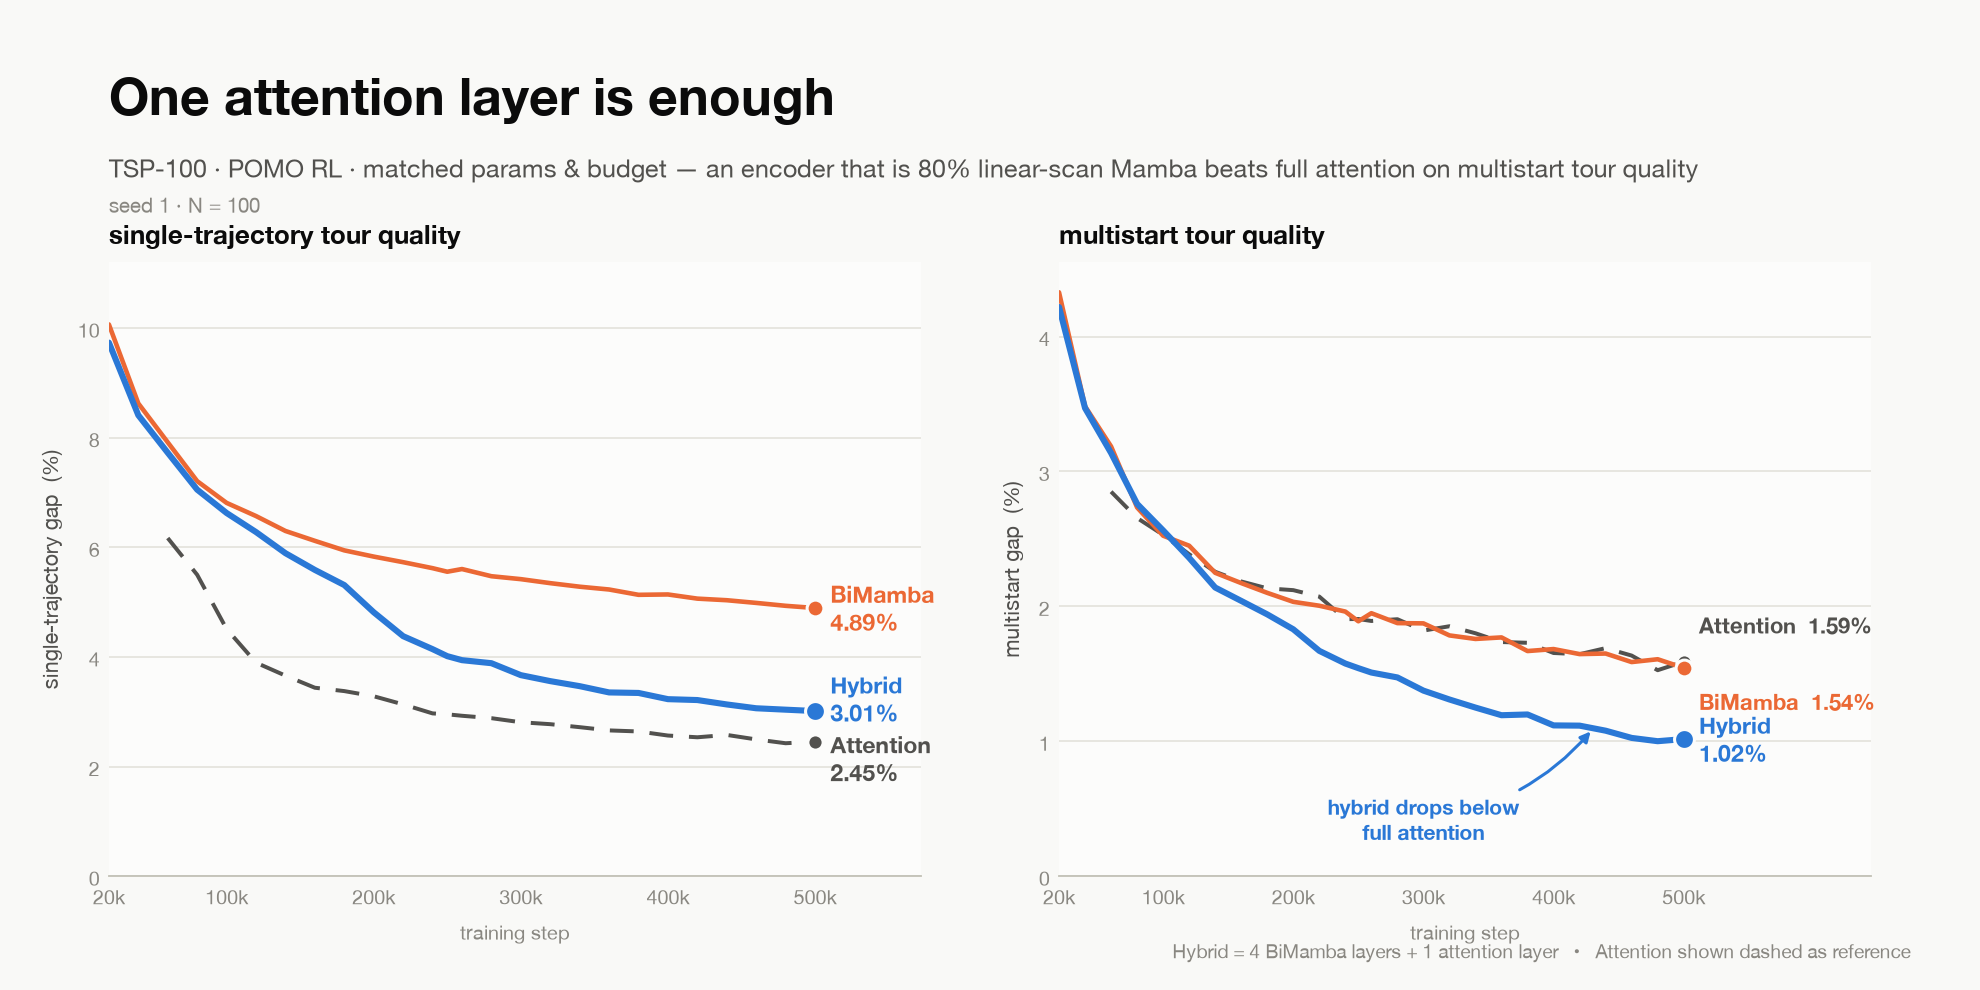
\includegraphics[width=0.9\linewidth]{figs/fig_hybrid_hero.png}
\caption{Hybrid encoder (4 bidirectional-Mamba layers + one attention layer,
4.5\pct{} fewer parameters than attention) versus the all-attention baseline.
At the converged 500k budget the hybrid beats attention on multistart tour
quality (\S\ref{sec:repair}), while attention remains ahead on
single-trajectory greedy decoding. All gaps are percent over the LKH-3 oracle.}
\label{fig:hero}
\end{figure}

\subsection{Best-of-$k$ serialization ensembling}
A scan encoder has a degree of freedom attention lacks: the serialization. At
inference on random-trained \emph{seed-1} checkpoints we draw $k=8$ random orders
and keep the per-instance best tour. This lowers uni-Mamba/random multistart from
3.33\pct{} to 2.72\pct{} (average-start 6.42\pct{}$\rightarrow$5.01\pct{}) and
BiMamba/random from 3.31\pct{} to 2.70\pct{} (the $k{=}1$ figures reproduce the
respective seed-1 training-time evals to within order-resampling noise; the
three-seed means in Table~\ref{tab:main} differ slightly). Attention has no ordering degree of freedom, so this is a
diversity knob unique to scan encoders. We report it as a supporting observation;
its natural host is a strong random-trained model, which---per \S\ref{sec:order}
---does not exist in the bidirectional regime.

% ============================================================================
% Tables: main 250k and converged 500k
% ============================================================================

\begin{table}[t]
\centering
\caption{Main results at the matched 250k-step budget. Optimality gap (\pct{}
over LKH-3), single-trajectory with multistart in parentheses; mean\,$\pm$\,std
over the noted seeds. Attention and multistart use no instance augmentation.
Every hybrid seed's multistart is below attention's 1.91.}
\label{tab:main}
\setlength{\tabcolsep}{5pt}
\begin{tabular}{ll cc}
\toprule
Encoder / order & Seeds & Single-traj (\pct{}) & Multistart (\pct{}) \\
\midrule
Attention             & s1        & 2.95              & 1.91 \\
\midrule
Uni-Mamba / Hilbert   & s1,s2,s3  & 7.50\,$\pm$\,1.03 & 3.64\,$\pm$\,1.09 \\
Uni-Mamba / random    & s1,s2,s3  & 6.90\,$\pm$\,0.53 & 3.28\,$\pm$\,0.14 \\
Uni-Mamba / sort      & s1        & 7.12              & 3.64 \\
\midrule
GC mean-pool ($+1.32\pct$)      & s1 & 7.86 & 4.13 \\
GC structured ($+2.62\pct$)     & s1 & 8.38 & 4.51 \\
\midrule
BiMamba / Hilbert     & s1,s2,s3  & 5.57\,$\pm$\,0.11 & 1.94\,$\pm$\,0.09 \\
BiMamba / random      & s1        & 7.61              & 3.30 \\
\midrule
Hybrid                & s1,s2,s3  & 4.37\,$\pm$\,0.33 & 1.63\,$\pm$\,0.10 \\
\bottomrule
\end{tabular}
\end{table}

\begin{table}[t]
\centering
\caption{Converged results at 500k steps (curves flat). Optimality gap (\pct{}
over LKH-3), single-trajectory (multistart). All rows are final 500k numbers;
the multistart eval-noise band is $\pm$0.05. The hybrid--attention multistart
separation is three-seed on both sides: worst hybrid 1.365 vs best attention
1.589.}
\label{tab:conv}
\setlength{\tabcolsep}{5pt}
\begin{tabular}{ll cc}
\toprule
Encoder & Seeds & Single-traj (\pct{}) & Multistart (\pct{}) \\
\midrule
Attention & s1              & 2.454 & 1.589 \\
Attention & s2              & 2.597 & 1.632 \\
Attention & s3              & 2.503 & 1.621 \\
Attention & s1,s2,s3 (mean) & 2.52\,$\pm$\,0.07 & 1.61\,$\pm$\,0.02 \\
\midrule
BiMamba / Hilbert & s1      & 4.893 & 1.544 \\
\midrule
Hybrid & s1                 & 3.013 & 1.016 \\
Hybrid & s2                 & 3.098 & 1.051 \\
Hybrid & s3                 & 3.136 & 1.365 \\
Hybrid & s1,s2,s3 (mean)    & 3.08\,$\pm$\,0.06 & 1.14\,$\pm$\,0.19 \\
\bottomrule
\end{tabular}
\end{table}

% ============================================================================
\section{Discussion and limitations}
\label{sec:discussion}
% ============================================================================

\paragraph{N$=$100 only; the $O(N)$ payoff is untested.}
Every number here is at N$=$100, where attention's $O(N^2)$ is cheap. The
motivation for a linear-scan encoder is large $N$, and our own geometry study
(\S\ref{sec:kill}) predicts the receptive-field deficit \emph{worsens} with scale.
Whether the hybrid's multistart advantage survives---and whether $O(N)$ actually
pays---at $N\geq1000$ is the next gate, not a claim of this paper.

\paragraph{Single-trajectory still favors attention.}
Our win is a multistart result. On single-trajectory greedy decoding attention
remains ahead at every budget we ran. A reader who cares about greedy decoding
should read this paper as parity-at-best for the state-space encoders.

\paragraph{The hybrid interleaving is prior art.}
Mixing attention layers into an SSM stack is established in language models
\citep{jamba2024,zamba2024} and local/global aggregation in point clouds
\citep{pillarmamba2025}. Our contribution is the RL-routing evidence and the
contrast we can draw because we ran both: one \emph{exact} attention layer works
where two pooled global-channel variants did not. That contrast, not the
architecture, is the result.

\paragraph{Fairness caveats.}
The 500k multistart comparison is three-seed on both sides: hybrid
1.14\,$\pm$\,0.19 versus attention 1.61\,$\pm$\,0.02, with the worst hybrid seed
(1.365) below the best attention seed (1.589). Attention at 250k remains a
single seed; there and wherever seed counts are unequal we report ranges and
worst-vs-best comparisons rather than significance tests. Multistart differences below
$\sim$0.05 are within eval noise and should not be read as wins. Finally, the
throughput table shows no speed advantage for the scan encoders at N$=$100
(bidirectional 4.78 vs attention $\sim$5.1 it/s): at this size the paper's
result is about \emph{quality at matched cost}, and the efficiency motivation
rests entirely on the untested N$\geq$1000 regime.

% ============================================================================
\section{Conclusion}
\label{sec:conclusion}
% ============================================================================

We set out to test whether a linear-time state-space encoder can route as well as
attention on TSP-100 under the reinforcement learning that NCO actually uses, with
the decoder and parameter budget held fixed. The vanilla Hilbert+Mamba recipe is
killed, and the failure is a short one-directional receptive field, not a bug or
collapsed representations. Following the diagnosis, pooled global channels do not
help, but bidirectionality reaches multistart parity with attention while cutting
seed variance tenfold, and a hybrid with a single exact attention layer---4.5\pct{}
smaller than the attention encoder---beats attention on converged multistart tour
quality. Along the way we found that the value of a serialization prior depends on
scan causality, and that a clean single-seed ordering curve was enough to state an
inversion two further seeds dissolved. All of this is scoped to N$=$100; whether
the linear-scan payoff materializes at larger $N$ is the open question we hand to
the next gate.\footnote{Code, seeds, the fixed evaluation set, and the
pre-registered decision rules are at
\url{https://github.com/Umaraslam66/serpentine}.}

% ============================================================================
\section*{Acknowledgments}
% ============================================================================
We gratefully acknowledge EuroHPC/CINECA for compute on the Leonardo Booster
partition (NVIDIA A100), under project AIFAC\_P02\_548.

% ============================================================================
\section*{Reproducibility}
% ============================================================================
All runs share a byte-identical POMO decoder, optimizer (Adam, lr
$1\times10^{-4}$, weight decay $1\times10^{-6}$), batch size 64, and gradient
budget (250k, 500k for extensions), on a single A100; only the encoder is
swapped. Evaluation uses a fixed 1000-instance held-out set with the LKH-3 oracle
mean $7.749371521$. The kill rule, the BiMamba three-bucket reading, and the
global-channel A/B rule were each written and committed \emph{before} the
corresponding runs. Code, seeds, curves, and the pre-registered rules are released at
\url{https://github.com/Umaraslam66/serpentine}. The mamba-ssm CUDA kernel was
gated against a pure-PyTorch reference at $<10^{-3}$ agreement.

\bibliographystyle{plainnat}
\bibliography{refs}

\end{document}
